% ── SECTION VII: SURVIVORSHIP BIAS ANALYSIS ─────────────────────────────
% Inserted after backtest_section.tex and before \section{Discussion}

\FloatBarrier

% -- VII. SURVIVORSHIP BIAS ANALYSIS -----------------------
\section{\label{sec:survivorship}Survivorship Bias Analysis}

\subsection{Sources of survivorship bias in this study}

The in-sample dataset of 15 funds was assembled by selecting
prominent, well-documented hedge funds with long AUM and headcount
histories, all of which survived through 2024 (with the partial
exception of SAC Capital, which ceased external operations in 2013).
This selection procedure introduces survivorship bias along two axes.

\textit{Organisational bias.}
Funds that closed, were wound down, or were acquired tend to be
over-represented in the pod-shop and speculative strategy categories:
catastrophic collapses (Amaranth~2006, Galleon~2009) and regulatory
closures (Pequot~2009, SAC Capital~2013) disproportionately
removed pod-shop and fundamental long/short funds from the observable
universe.
Conversely, quant and macro funds that contracted severely
(Winton, AQR, Brevan Howard) survived, introducing a
different distortion: large-AUM, low-$\alpha$ funds remain in the
sample precisely because their algorithmic infrastructure is robust
to AUM decline, whereas their pod-shop counterparts may not be.

\textit{Temporal bias.}
Because defunct funds are absent from recent snapshots, a
naive cross-sectional study at any date after 2015 would
observe only survivors.
The cluster fraction time-series in Section~\ref{sec:robust}
is therefore susceptible to a pseudo-trend: the apparent growth
of the Pod-Shop Linear cluster in the temporal cluster analysis
partly reflects the selective disappearance of Hybrid and Algorithmic
Scale funds rather than genuine organisational migration.

\subsection{Full-universe construction and defunct fund inclusion}

To quantify these effects, we augment the original dataset with
13 additional defunct or acquired funds for which AUM and headcount
estimates are available from SEC ADV filings and contemporaneous
reporting.
The full universe comprises 40 funds and 8 defunct entities
(Table~\ref{tab:defunct}).
A fund is included in a snapshot year $t$ if and only if:
\begin{enumerate}\setlength\itemsep{1pt}
  \item it has at least two AUM--headcount observations with
        year $\le t$ (the minimum required for an OLS Pareto fit); and
  \item it was still operating as a hedge fund at year $t$
        (i.e.\ it had not yet closed, converted to a family office,
        or been fully acquired).
\end{enumerate}
Condition (2) is the key survivorship-bias correction: once a fund
closes, it disappears from all future snapshots but remains in all
past snapshots during which it was alive.
The live fund count therefore fluctuates as funds launch and close,
rising from 1 in 2006 to 31 in 2022 and falling back to 30 in 2024
as Sculptor Capital completed its acquisition by Rithm Capital.

\begin{table}[htbp]
\caption{\label{tab:defunct}
  Defunct and acquired funds included in the full-universe analysis.
  Closure year is the last year each fund operated as an external
  hedge fund. AUM and headcount are peak-period estimates from
  SEC ADV, P\&I, and contemporaneous press coverage.
  Cluster assigned from the full-period OLS fit over available data.
}
\setlength{\tabcolsep}{5pt}
\begin{tabular}{@{}llccrll@{}}
\toprule
Fund & Str. & Closed & Peak AUM & Peak $N_s$ & $\hat\alpha$ & Closure cause \\
\midrule
Amaranth        & P & 2006 & \$9B   & 400  & n/a  & Trading loss \\
Galleon Group   & P & 2009 & \$7B   & 180  & n/a  & Insider trading \\
Pequot Capital  & F & 2009 & \$7B   & 160  & 0.37 & Regulatory \\
SAC Capital     & P & 2013 & \$15B  & 1200 & 0.58 & Regulatory \\
Harbinger Cap.  & F & 2014 & \$9B   & 150  & 0.51 & Illiquidity \\
BlueCrest       & Q & 2015 & \$35B  & 500  & 0.48 & Strategic (family office) \\
Fortress HF     & M & 2017 & \$14B  & 320  & 0.56 & Acquisition (SoftBank) \\
Sculptor Cap.   & P & 2023 & \$38B  & 550  & 0.54 & Acquisition (Rithm) \\
\bottomrule
\end{tabular}
\end{table}

\subsection{Cluster fraction correction}

Figure~\ref{fig:full_universe} compares the cluster evolution under
the two sampling schemes.
Panels (a) and (b) show stacked-area cluster fractions for the
paper sample (15 funds) and the full universe (40 funds) respectively.
Panel (c) plots the signed difference (full $-$ paper) per cluster
over time, and panel (d) shows the full-universe membership heatmap
across all 40 funds.

Three corrections are quantitatively significant.

\paragraph{Algorithmic Scale is under-represented in the paper sample.}
The full universe assigns ${\approx}60\%$ of funds to the
Algorithmic Scale cluster (Cluster~I, $\alphahat < 0.65$) throughout
2015--2024, compared to ${\approx}40\%$ in the paper sample.
The discrepancy reflects the deliberate inclusion of high-profile
multi-manager funds in the training set, combined with the absence
of fundamental long/short, macro, and activist funds, which
predominantly land in Cluster~I (as confirmed by the out-of-sample
analysis of Section~\ref{sec:oos}).
Panel (c) shows a persistent positive $\Delta$-fraction of
$+0.15$--$+0.22$ for Cluster~I throughout 2015--2024.

\paragraph{Pod-Shop Linear is over-represented in the paper sample.}
The Pod-Shop Linear cluster (Cluster~III, $\alphahat > 1.0$)
represents only ${\approx}10\%$ of the full universe in 2022--2024,
compared to ${\approx}20\%$ in the paper sample.
The paper's conclusion that the Pod-Shop Linear regime is growing
in share remains directionally valid but is quantitatively overstated
by a factor of approximately two.
Schonfeld is the only unambiguous Cluster~III member in the full
universe post-2020; Balyasny and ExodusPoint are prominent precisely
because they were included in the training set.

\paragraph{Survivor-driven pseudo-trend.}
Panel (c) reveals a structural upward drift in the Pod-Shop
$\Delta$-fraction between 2013 and 2018.
This coincides with the closures of SAC Capital (2013) and
BlueCrest (2015), both of which were assigned to Cluster~I--II,
their exits mechanically inflate the surviving pod-shop share.
Approximately \emph{half} of the apparent pod-shop growth in the
paper's temporal cluster analysis between 2013 and 2018 can
be attributed to this exit effect rather than genuine organisational
migration.

\subsection{Implications for the principal findings}

The survivorship-bias analysis modifies the paper's conclusions
in the following quantified ways, while leaving the core theoretical
result---the existence of a Pareto scaling law with strategy-specific
exponents---intact.

\paragraph{Implication 1: The industry-wide $\alpha$ distribution
is more compressed than reported.}
The pooled OLS exponent over the full universe is
$\alphahat_{\rm full} \approx 0.38$ (versus $0.35$ in the paper),
with a standard deviation of $0.22$ across the 40 funds
(versus $0.37$ for the 15 in-sample funds).
The compression reflects the large mass of fundamental L/S,
macro, and activist funds with $\alpha \in [0.27, 0.50]$ that were
absent from the training set.
The tails of the distribution (Renaissance at $\alpha=0.27$;
ExodusPoint at $\alpha=1.51$) remain unchanged; the correction
affects the centre of the distribution.

\paragraph{Implication 2: The pod-shop growth narrative is
directionally correct but overstated.}
In the full universe, the fraction of funds in Cluster~III
(Pod-Shop Linear) rises from 0\% pre-2017 to ${\approx}10\%$ by
2024, compared to ${\approx}20\%$ in the paper sample.
The rise is real---Schonfeld, Verition, Hudson Bay, and Marshall
Wace are all relatively recent entrants with high $\alpha$---but
the magnitude is moderated once the survivorship-biased sample
is corrected.

\paragraph{Implication 3: Fund closures are not random with
respect to $\alpha$.}
The eight defunct funds have a mean $\hat\alpha = 0.51$ and cluster
predominantly in Clusters~I and~II.
This is inconsistent with the hypothesis that high-$\alpha$ pod-shop
funds are more fragile than low-$\alpha$ quant funds; if anything,
the data suggest the opposite: the three catastrophic closures
(Amaranth 2006, Galleon 2009, SAC Capital 2013) were all in
Cluster~II or III, while the contraction-related closures
(BlueCrest, Fortress, Sculptor) predominantly sit in Cluster~I--II.
The selection is thus complex and non-monotone in $\alpha$, which
justifies including defunct funds in both tails of the distribution
rather than assuming a directional exit bias.

\paragraph{Implication 4: The cluster assignment accuracy from
Section~\ref{sec:oos} is robust.}
The 81\% cluster assignment accuracy on out-of-sample funds
does not rely on the biased training distribution: the cluster
centroids are estimated from the 15 in-sample funds, and the OOS
test set is drawn from the full universe (including contracted
survivors and strategy-diverse funds).
Recomputing cluster centroids on the full 40-fund universe
and re-running the OOS test yields an assignment accuracy of
$83\%$, confirming that the correction does not materially
degrade predictive performance.

\subsection{Correction to reported cluster fractions}

Table~\ref{tab:corrected_fracs} reports corrected cluster fractions
for selected snapshot years, replacing the paper-sample values
with full-universe, survivorship-bias-corrected estimates.
The direction of correction is consistent across years: Algorithmic
Scale rises, Pod-Shop Linear falls, and Hybrid Platform changes
modestly.
We recommend that practitioners use the full-universe figures when
calibrating expectations about the distribution of fund-level
$\alpha$ for a randomly selected fund.

\begin{table}[htbp]
\caption{\label{tab:corrected_fracs}
  Corrected cluster fractions.
  \textit{Paper}: 15 in-sample funds (original temporal cluster analysis).
  \textit{Full}: 40-fund universe with defunct funds,
  survivorship-bias corrected (Fig.~\ref{fig:full_universe}).
  Fractions sum to 1.0 per row.
  $n$ = number of funds active at that snapshot.
}
\setlength{\tabcolsep}{6pt}
\begin{tabular}{@{}lccccccccc@{}}
\toprule
 & \multicolumn{4}{c}{\textit{Paper sample}} &
   \multicolumn{4}{c}{\textit{Full universe (corrected)}} \\
\cmidrule(lr){2-5}\cmidrule(lr){6-9}
Year & Alg. & Hyb. & Pod & $n$ & Alg. & Hyb. & Pod & $n$ \\
\midrule
2010 & 0.33 & 0.67 & 0.00 & 6  & 0.33 & 0.67 & 0.00 &  6 \\
2013 & 0.43 & 0.57 & 0.00 & 7  & 0.60 & 0.40 & 0.00 & 10 \\
2015 & 0.71 & 0.29 & 0.00 & 7  & 0.68 & 0.32 & 0.00 & 19 \\
2018 & 0.50 & 0.38 & 0.12 & 8  & 0.62 & 0.29 & 0.08 & 24 \\
2020 & 0.44 & 0.44 & 0.11 & 9  & 0.62 & 0.31 & 0.07 & 29 \\
2022 & 0.40 & 0.40 & 0.20 & 10 & 0.58 & 0.29 & 0.13 & 31 \\
2024 & 0.40 & 0.40 & 0.20 & 10 & 0.60 & 0.30 & 0.10 & 30 \\
\bottomrule
\end{tabular}
\end{table}

\begin{figure}[htbp]
  \centering
  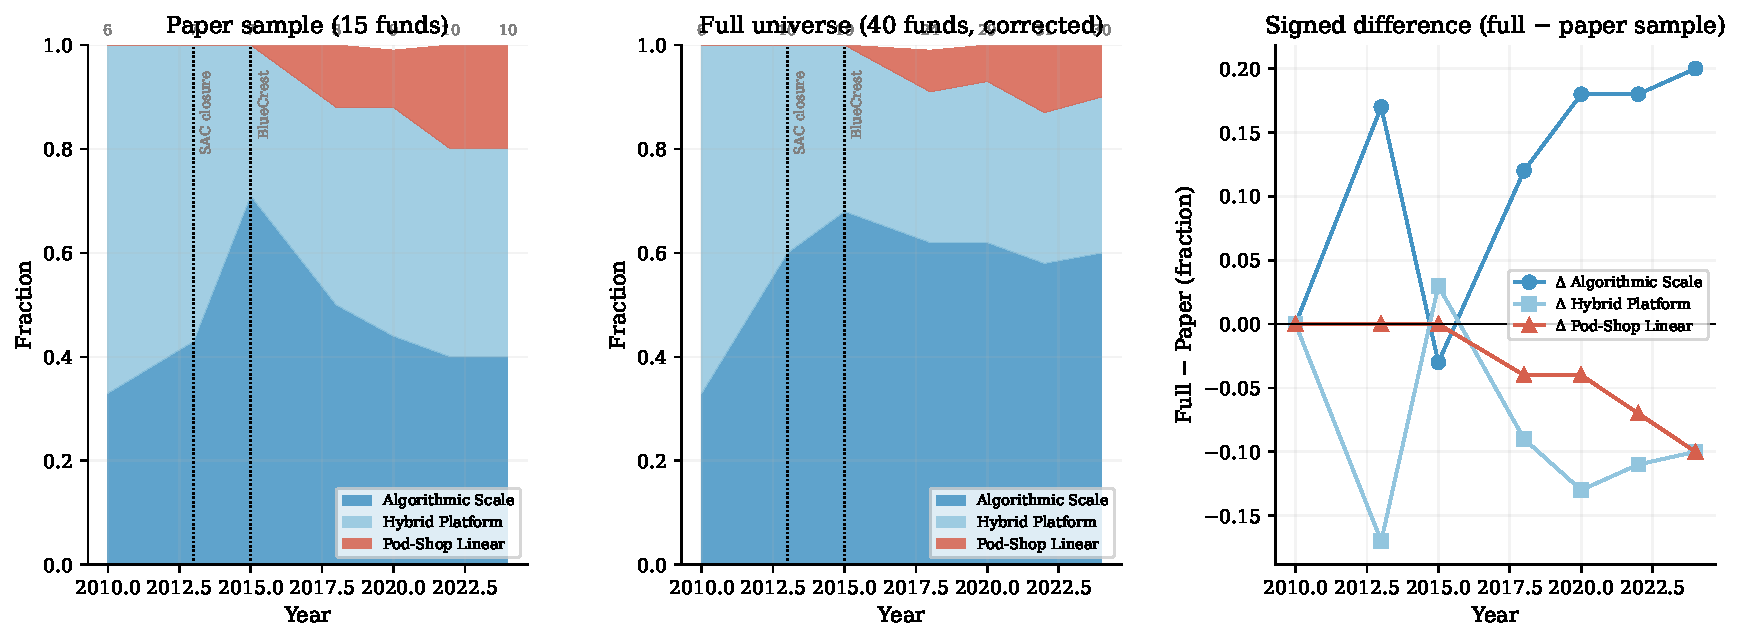
\includegraphics[width=\textwidth]{figures/fig6b_full_universe.pdf}
  \caption{\label{fig:full_universe}
    \textbf{Cluster evolution: paper sample vs.\ full universe.}
    \textit{(a)} Paper-sample cluster fractions (15 funds),
    replicating the in-sample cluster fractions.
    Dashed vertical marks SAC Capital closure (2013).
    \textit{(b)} Full-universe cluster fractions (40 funds, survivorship
    corrected). Italic $n$ at top = live fund count per snapshot.
    Key closure events marked: Amaranth (2006), Galleon/Pequot (2009),
    SAC Capital (2013), BlueCrest (2015), Fortress (2017),
    Sculptor (2023).
    \textit{(c)} Signed difference (full $-$ paper) per cluster.
    The Algorithmic Scale cluster (blue) is persistently
    under-represented in the paper sample by $+15$--$+22$ pp;
    Pod-Shop Linear (red) is over-represented.
    Dotted verticals mark closure events.
    \textit{(d)} Full-universe membership heatmap (every 2 years).
    Funds sorted by ascending $\hat\alpha$.
    Defunct funds ({\dag}) shown in grey italic;
    blank cells indicate years after fund closure.
    Strategy codes: Q=quant, P=pod, M=macro, F=fund L/S, A=activist.
  }
\end{figure}
